\section{Kostenrechnung}
Übersicht: s. FS4/13
\subsection{Kostenartenrechnung}
\textbf{Frage}: Welche Kosten sind in welcher Höhe in einer Periode angefallen? 
$\rightarrow$ Aufteilung auf Kostenarten

\textbf{Kostenarten}: Kategorie von Kosten, die nach bestimmten Kriterien aufgegliedert werden können

\textbf{Kostenartenhauptgruppen}: Personal- und Sozialkosten, Sach- und Materialkosten
Dienstleistungskosten, Kosten für Lizenzen, Kapitalkosten, öffentliche Abgaben und Steuern, Versicherungskosten und kalkulatorische Wagniskosten

\textbf{Variable Kosten}: Kosten, die mit der Ausprägung (Stückzahl) eines Kostentreibers variieren

\textbf{Fixe Kosten}: Kosten, die unabhängig vom Kostentreiber immer in konstanter Höhe anfallen

\textbf{Kostentreiber}: Variable, die am besten erklärt, wie die gesamten Kosten eines Kostenobjektes zustande kommen, z.B. Produktionsvolumen, Lieferungen, $\ldots$

\textbf{Break-even-Analyse}:
\begin{center}
	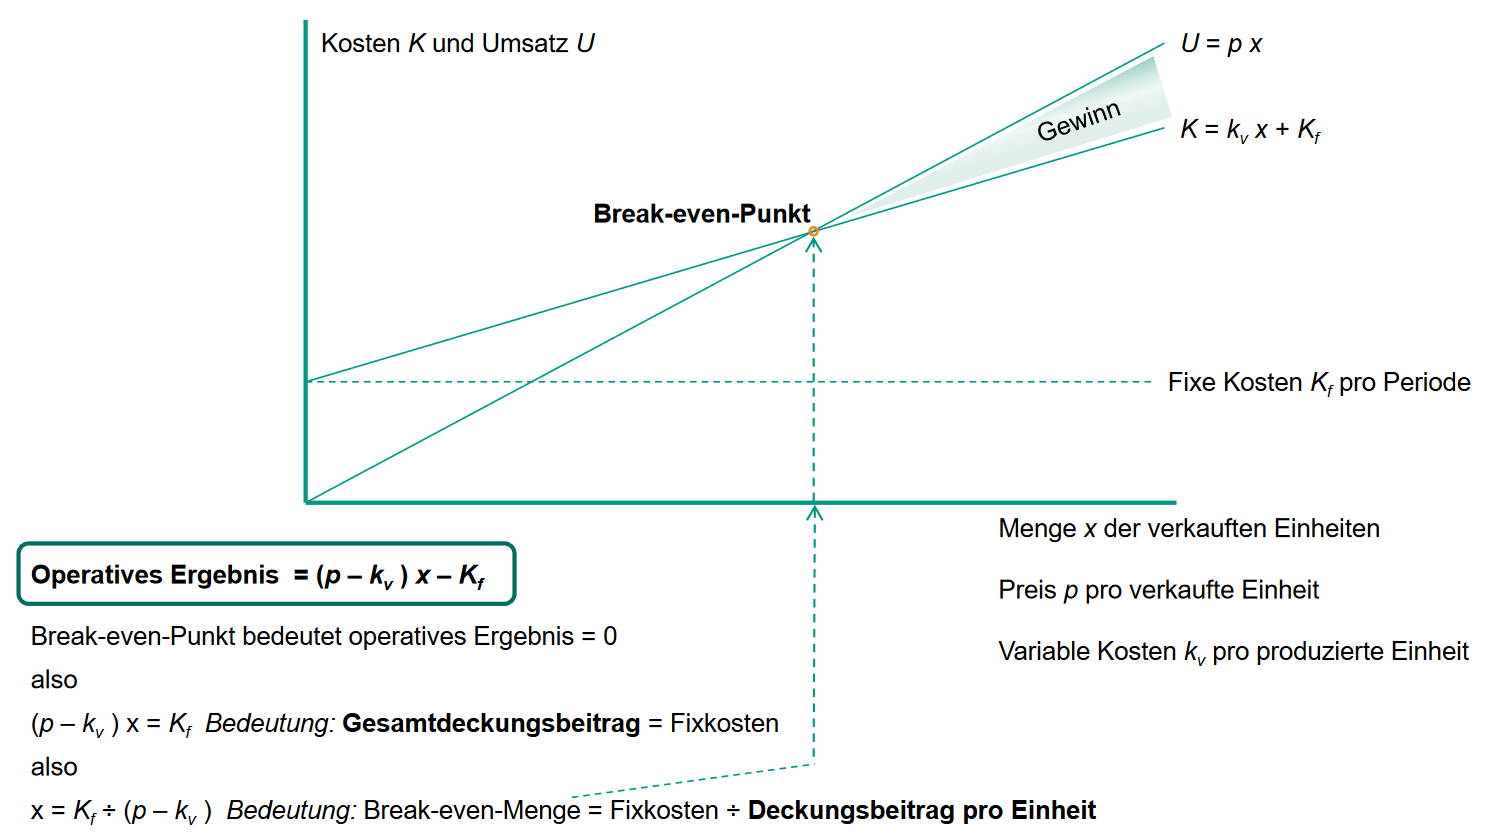
\includegraphics[width=\textwidth]{images/be-analyse.png}
\end{center}
$\text{Gewinn}=p\cdot x-k_V\cdot x-K_f$ \qquad\qquad\qquad\qquad\qquad\qquad\textit{Bsp. s. FS4/21}
\bigskip

\textbf{Einzelkosten}: Können einem Kostenobjekt (Kostenträger) eindeutig und vollständig zugeordnet werden

\textbf{Gemeinkosten}: Werden durch mehrere Kostenobjekte gemeinsam erzeugt $\rightarrow$ müssen indirekt über sinnvolle Kostenverteilungsschlüssel aufgeteilt werden

\textbf{Kostenobjekt}: Alles, wonach die Frage nach Kosten Sinn ergibt, z.B. Auftrag, Dienstleistung, Kunde, Standort.\\
$\rightarrow$ Einteilung in variable/fixe/Einzel-/Gemeinkosten nicht immer eindeutig!

\textbf{Ist-Kosten}: Bisher tatsächlich angefallene Kosten

\textbf{Plan-Kosten}: Zukünftig zu erwartende Kosten

\textbf{Normalkosten}: Durchschnittliche Ist-Kosten mehrerer vergangener Perioden

\subsection{Kostenstellenrechnung}
\textbf{Frage}: Wo fallen die Kosten an?

\textbf{Kostenstelle}: Organisatorischer Bereich, für den Kosten selbständig geplant, erfasst und
kontrolliert wird

\textbf{Kostenstellenhauptgruppen}: Fertigungsstellen, Materialstellen, Verwaltungsstellen, Vertriebsstellen, Forschungs- und Entwicklungsstellen, Allgemeine (Hilfs-)Stellen
\begin{itemize}
	\item \textbf{Vorkostenstellen}: Für interne Verwaltung und Dienstleistungen
	\item \textbf{Endkostenstellen}: Arbeit an Kostenobjekten, die Kunden kaufen
\end{itemize}

\textbf{Ziel der Kostenstellenrechnung}: Aufgliederung der Kostenarten auf Kostenstellen
\begin{itemize}
	\item \textbf{Primärkostenverrechnung}: Zuordnen und Verteilen der Kosten auf Kostenstellen
	\begin{itemize}
		\item \textbf{Produkt-Einzelkosten}: Eindeutig einem Produkttyp, also einem Kostenträger zuordenbar
		\item \textbf{Kostenstelle-Einzelkosten}: Eindeutig einer Kostenstelle zuordenbar (aber keinem Produkttyp)
		\item \textbf{Kostenstellen-Gemeinkosten}: Entstehen für mehrere Kostenstellen und müssen über geeignete Schlüssel auf Kostenstellen verteilt werden
	\end{itemize}
	\item \textbf{Sekundärkostenrechnung}: Verteilen der Kosten von Vorkostenstellen auf Endkostenstellen
	\begin{itemize}
		\item \textbf{Anbauverfahren}: Kosten der Vorkostenstellen werden nur auf Endkostenstellen verteilt, aber nicht auf andere Vorkostenstellen
		\item \textbf{Stufenleiterverfahren}: Kosten der Vorkostenstellen werden auf Endkostenstellen und auch auf andere Vorkostenstellen verteilt (aber nur in eine Richtung!)\\
		$\rightarrow$ Reihenfolge hat Einfluss auf Berechnung\\
		$\rightarrow$ Starte mit Kostenstelle, die prozentual am meisten Leistungen für andere Vorkostenstellen erbringt
		\item \textbf{Gleichungsverfahren}: Wie Stufenleiterverfahren, aber zwei Vorkostenstellen können sich auch wechselseitig mit Kosten belasten
	\end{itemize}
	$\rightarrow$ \textbf{Gesamtkosten pro Kostenstelle} = Kostenstelle-Einzelkosten + primäre zugerechnete Gemeinkosten + sekundär zugerechnete Gemeinkosten\\
	$\rightarrow$ Wahl der Methode abhängig von Unternehmensstruktur
\end{itemize}
\textit{s. Gleichungen FS5/23-28!!!}\\

\textbf{Betriebsabrechnungsbogen (BAB)}: Werkzeug für Kostenstellenrechnung
\begin{itemize}
	\item Spalten $\widehat{=}$ Kostenstellen
	\item Zeilen $\widehat{=}$ Kosten je Kostenstelle
	\item $\sum\text{Horizontal }\widehat{=}$ Kostenentlastung der leistenden Kostenstelle
	\item $\sum\text{Vertikal }\widehat{=}$ Gesamtkosten der Kostenstelle
\end{itemize}
\textit{s. Bsp. FS5/21}

\subsection{Kostenträgerrechnung}
\textbf{Frage}: Wofür fallen die  Kosten an?

\textbf{Kostenträger}: Kostenobjekt, an dem das Unternehmen die Kosten festmachen will, um festzustellen, wie gewinnbringend dieses Objekt ist

\textbf{Prinzipien der Kostenverteilung}:
\begin{itemize}
	\item \textbf{Verursachungsprinzip}: Auf Kostenobjekte verteilen, die ursächlich für die
	Kostenentstehung sind
	\item \textbf{Durchschnittsprinzip}: Pauschal auf Kostenobjekte verteilen, wenn der
	Kostentreiber nicht bekannt ist
\end{itemize}

\textbf{Methoden der Kostenträgerstückrechnung}:
\begin{itemize}
	\item Divisionskalkulation
	\item Äquivalenzziffernkalkulation
	\item Zuschlagskalkulation
	\item Maschinenstundensatzkalkulation
	\item Lohnstundensatzkalkulation
\end{itemize}
\bigskip
\textbf{Divisionskalkulation}:
\begin{itemize}
	\item \textbf{Einstufige Divisionskalkulation}: $\text{Selbstkosten pro Stück}=\cfrac{\text{Gesamtkosten}}{\text{Produktionsmenge}}$
	
	Voraussetzungen: 
	\begin{enumerate}
		\item Unternehmen mit homogenen Massenprodukten, z.B. Strom
		\item Keine (schwankende) Lagerhaltung unfertiger + fertiger Erzeugnisse
	\end{enumerate}

	\item \textbf{Zweistufige Divisionskalkulation}: Bei Lagerung fertiger Erzeugnisse
	\begin{tightcenter}
		$\text{Selbstkosten pro Stück}=
		\cfrac{\text{Herstellkosten}}{\text{Produktionsmenge}}+
		\cfrac{\text{Verwaltungs- und Vertriebskosten}}{\text{Absatzmenge}}$
	\end{tightcenter}
	\item Wenn auch unfertige Erzeugnisse gelagert werden $\rightarrow$ \textbf{mehrstufige Divisionskalkulation}
\end{itemize}
\bigskip
\textbf{Äquivalenzziffernkalkulation}: Verwandte, ähnliche Produkte werden über Äquivalenzziffern in ein \enquote{Einheitsprodukt} umgerechnet
\begin{enumerate}
	\item Einem Produkt wird die Äquivalenzziffer 1 zugeordnet
	\item Äquivalenzziffer der anderen Produkte anhand von deren Aufwand schätzen (Je komplexer, desto größere ÄZ)
	\item Berechne Gesamteinheitsmenge: $\sum\text{ÄZ}_i\cdot x_i$, wobei $x_i$ die Menge an Produkt $i$ ist
	\item Stückselbstkosten des Einheitsproduktes ermitteln: $\cfrac{\text{Gesamtkosten}}{\text{Gesamteinheitsmenge}}$
	\item Ermittlung der Stückkosten der äquivalenten Produkte:
	\begin{tightcenter}
		$\text{ÄZ}_i\cdot \text{Stückselbstkosten des Einheitsproduktes}$
	\end{tightcenter}
\end{enumerate}
\textit{s. FS6/7-8}\\

\textbf{Zuschlagskalkulation}: